In this final section we present a formal specification of some of the requirements explained before. Using the Alloy analyzer we provide a description of the model and we try to prove its correctness and consistency. In particular, we show some constraints of the world in which the system to be will operate, and some functionalities. The objective driving this modeling phase was to verify that the model we have in mind regarding bookings and charging sessions respect the main overlapping constraints of the world. At the end of this section we also provide some visualizations of the obtained result, further explaining the satisfied requirements.

\begin{lstlisting}[frame = single]
open util/ordering[DateTime]

sig DateTime{}

// some actors in the system
abstract sig User {}

//We don't consider dangling elements 
sig Email{}{
	this in EVD.email
}
sig Password{}{
	this in EVD.password
}
sig Location{}{
	this in ChargingStation.location
}
sig History{
}{
	this in EVD.chargingHistory
}

sig EVD {
	evs: some EV,
    email: one Email, 
	password: one Password,
	chargingHistory: one History
}

sig DSO {}{
	this in ChargingStation.dso
}

abstract sig Socket {}
one sig Type1, Type2, Chademo extends Socket{}

sig EV {
	socket: one Socket,
}{
	this in EVD.evs
}

sig ChargingPoint {
 	socket: some Socket,
	connectedEV: lone EV
}{
	EV.socket in socket
	this in ChargingStation.chargingPoints
}

sig ChargingStation {
	chargingPoints: some ChargingPoint,
	location: one Location,
	dso: one DSO
}{
	this in CPO.chargingStations
}

sig CPO extends User{
	chargingStations: some ChargingStation
}

sig Booking {
	ev: EV,
	cs: ChargingStation,
	cp: ChargingPoint,
	start: DateTime,
	end: DateTime
}{
	// Only Registerd User can book
	ev in EVD.evs &&
	cp in cs.chargingPoints
	lt[start, end]
}

/*********** FACTS  *************/
//A charging point can belong only to a charging station
fact eachChargingToOnlyOneChargingStation{
	all disj x, y : ChargingStation |
		 #(x.chargingPoints & y.chargingPoints) = 0
}

//A charging station can be managed only by a CPO
fact eachCStoOnlyOneCPO{
	all disj x, y : CPO |
		 #(x.chargingStations & y.chargingStations) = 0
}

//An EV can belong to only an EVD
fact eachEVtoOnlyOneEVD {
	all disj x, y : EVD |
		 #(x.evs & y.evs) = 0
}

//The EV in a certain moment can be connected to only a charging point to charge
fact eachEVConnectedToOneChargingPoint{
    all disj x, y: ChargingPoint |
		 #(x.connectedEV & y.connectedEV) = 0
}

//Impose that there must not exist multiple bookings for the same vehicles at the same time
fact noEVOverBooking{
	no disj b1, b2: Booking
	| b1.ev = b2.ev && 
 		(gte[b1.start, b2.start] && lte[b1.start, b2.end] ||
 		 gte[b1.end, b2.start] && lte[b1.end, b2.end])
}

//Impose that there must not exist multiple bookings for the same charging point at the same time
fact noOverBooking{
	no disj b1, b2: Booking
	| b1.cp = b2.cp && 
		(gte[b1.start, b2.start] && lte[b1.start, b2.end] ||
		 gte[b1.end, b2.start] && lte[b1.end, b2.end])
}

//Only an EV can be in charge for an EVD in a certain moment
fact onlyAnEVisChargingForEVD{
	all evd: EVD, disj ev1, ev2 :EV |
	ev1 in evd.evs and ev2 in evd.evs and ev1 in ChargingPoint.connectedEV
	implies ev2 not in ChargingPoint.connectedEV
}

//Unique email to EVD
fact uniqueEmail{
 no disj driver1, driver2: EVD |
 	 driver1.email = driver2.email 
}

//Unique history to EVD
fact uniqueHistory{
 no disj driver1, driver2: EVD |
 	 driver1.chargingHistory = driver2.chargingHistory
}

//Unique location to ChargingStation
fact uniqueLocation{
 no disj cs1, cs2: ChargingStation |
 	 cs1.location = cs2.location
}

/**** ASSERTIONS ****/
//The same charging point can't be in two different charging stations
assert noCPinTwoChargingStations{
	no cp: ChargingPoint, disj cs1, cs2: ChargingStation | 
		cp in cs1.chargingPoints && cp in cs2.chargingPoints
}

//The same charging station can't be managed by two different CPOs
assert NoCSInTwoCPO{
 no cs: ChargingStation, disj CPO1, CPO2: CPO |
	cs in CPO1.chargingStations && cs in CPO2.chargingStations
}

//There is no charging point that doesn't belong to a charging station, because it's an entity that doesn't exist on its own in our system
assert notExistsCPnotInCS{
	no cp: ChargingPoint
	| cp not in ChargingStation.chargingPoints
}

//There is no EV that doesn't belong to a EVD, because it's an entity that doesn't exist on its own in our system
assert existsEVnotInRegEVD{
	some ev: EV
	| ev not in EVD.evs
}

//The booking has to regard an EV that belongs to the EVD, so an unregistered EVD cannot use this functionality, because the system is not able to keep track of its vehicles, and furthermore we also check that a booking cannot regard an EV that doesn't exist in the list of vehicles of the EVD
assert noBookingForUnregEVD{
	Booking.ev in EVD.evs
}

//There are no overlapping bookings for the same vehicle
assert noEVOverBooking{
	no disj b1, b2: Booking |
	b1.ev = b2.ev && gte[b1.start, b2.start] && lte[b1.start, b2.end]
}

//There are no overlapping bookings for the same charging point in the system, to maintain consistency and assure a correct service
assert bookingStartLessThanBookingEnd{
	all b: Booking | lt[b.start, b.end]
}

//Using the check we can see if Alloy finds some counterexamples of an assertion, checking the consistency of the world
check noCPinTwoChargingStations

/*********PREDICATES*********/
pred findBookings{
	some disj b1, b2: Booking | lt[b2.end, b1.start]
}

//Is possible to add an EV to the EVD
pred addEVToEVD[evd', evd: EVD, NewEv: EV]{
	evd'.evs = evd.evs + NewEv
}

//Is possible to add a charging station to the ones managed by a CPO
pred addCSToCPO[cpo', cpo: CPO, NewCS: ChargingStation]{
    cpo'.chargingStations = cpo.chargingStations + NewCS
}

//Is possible to delete a charging station from the ones managed by a CPO
pred deleteCSFromCPO[cpo', cpo: CPO, cs: ChargingStation]{
    cpo'.chargingStations = cpo.chargingStations - cs
}

//Is possible to add a charging point to a charging station, related to the CPO that manages it
pred addCPToCS[cs', cs:ChargingStation, cp: ChargingPoint, cpo, cpo': CPO]{
	cs in cpo.chargingStations
    cs'.chargingPoints = cs.chargingPoints + cp
	cpo'.chargingStations = cpo.chargingStations + cs'
}

//We show the task that the CPO wants to perform on the charging station, adding a new charging point, showing the case in which we already have other charging points, so we are not initializing the charging station, we are just updating it with new information
pred showAddCPToCS [cs', cs:ChargingStation, cp: ChargingPoint, cpo, cpo': CPO]{
	addCPToCS[cs', cs, cp, cpo, cpo']
	#(cs'.chargingPoints) > 2
}

//Dynamic model
run showAddCPToCS for 20 but exactly 3 ChargingStation

//To show the CPO interaction with the system
pred CPOworld{
	#CPO >= 2
	#ChargingStation >= 2
	#ChargingPoint >= 5
}

run CPOworld for 20

//To show the RegEVD interaction with the system
pred EVDworld{
	#EVD >= 2
	#EV >= 3
	#ChargingPoint >= 2
	#ChargingStation >= 1
	#Booking >= 1
}

run EVDworld for 10

run {} 
\end{lstlisting}

%TODO: a little explanation for each world important elements
\subsection{Resulting worlds}
\paragraph{The world mainly from the CPO point of view}
From the CPO point of view we show the following world generated with the Alloy analyzer, noticing some important requirements of the eMall:
\begin{itemize}
    \item The CPO manages one or more charging stations
    \item The charging stations have one ore more charging points
    \item The charging points can have different socket types (in the following representation Alloy generated a case in which each charging point has only a socket of one type, but in general the charging point can have many sockets of different types, but we assume that only one is used at the time)
    %TODO: add assumption only a socket is used at the time
    \item The charging stations acquire energy from different DSOs chosen by the CPO, and different charging stations, even of different CPOs, can acquire energy from the same DSO 
\end{itemize}
We can see a simple representation of these elements in the CPOworld:
\begin{figure}[H]
    \centering
    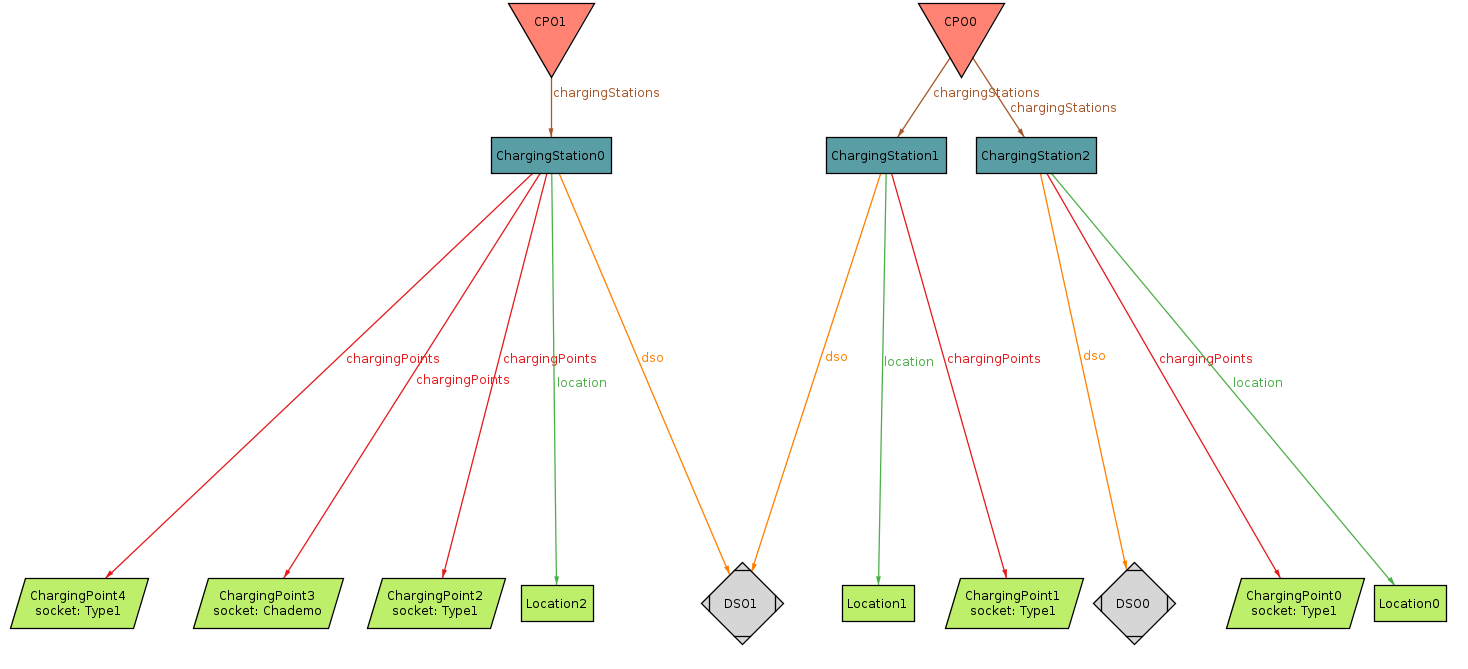
\includegraphics[width=1\textwidth]{Images/cp4/CPOWorld.png}
    \caption{A representation of the world from the CPO point of view}
\end{figure}

%TODO: in the Alloy connect the history with the chargings and the bookings
\paragraph{The world mainly from the EVD point of view}
To represent the EVD point of view we show a couple of worlds generated by the Alloy analyzer, in order to verify some requirements: 
\begin{itemize}
    \item The EVD has a mail and a password that he uses to log in
    \item The EVD has a charging history of his activities
    \item The EVD has one or more EVs, at least one because we assume that during registration phase the driver inserts a vehicle
    \item The EVD can have one or more bookings regarding an EV, but without overlapping time-frames
    \item There can be more bookings for a charging point, but without overlap in the time-frame chosen for the charging session
    \item An EVD can use the charging points, even without a booking
\end{itemize}

In the following two representations we can notice that the elements just explained are present and satisfied.
\begin{figure}[H]
    \centering
    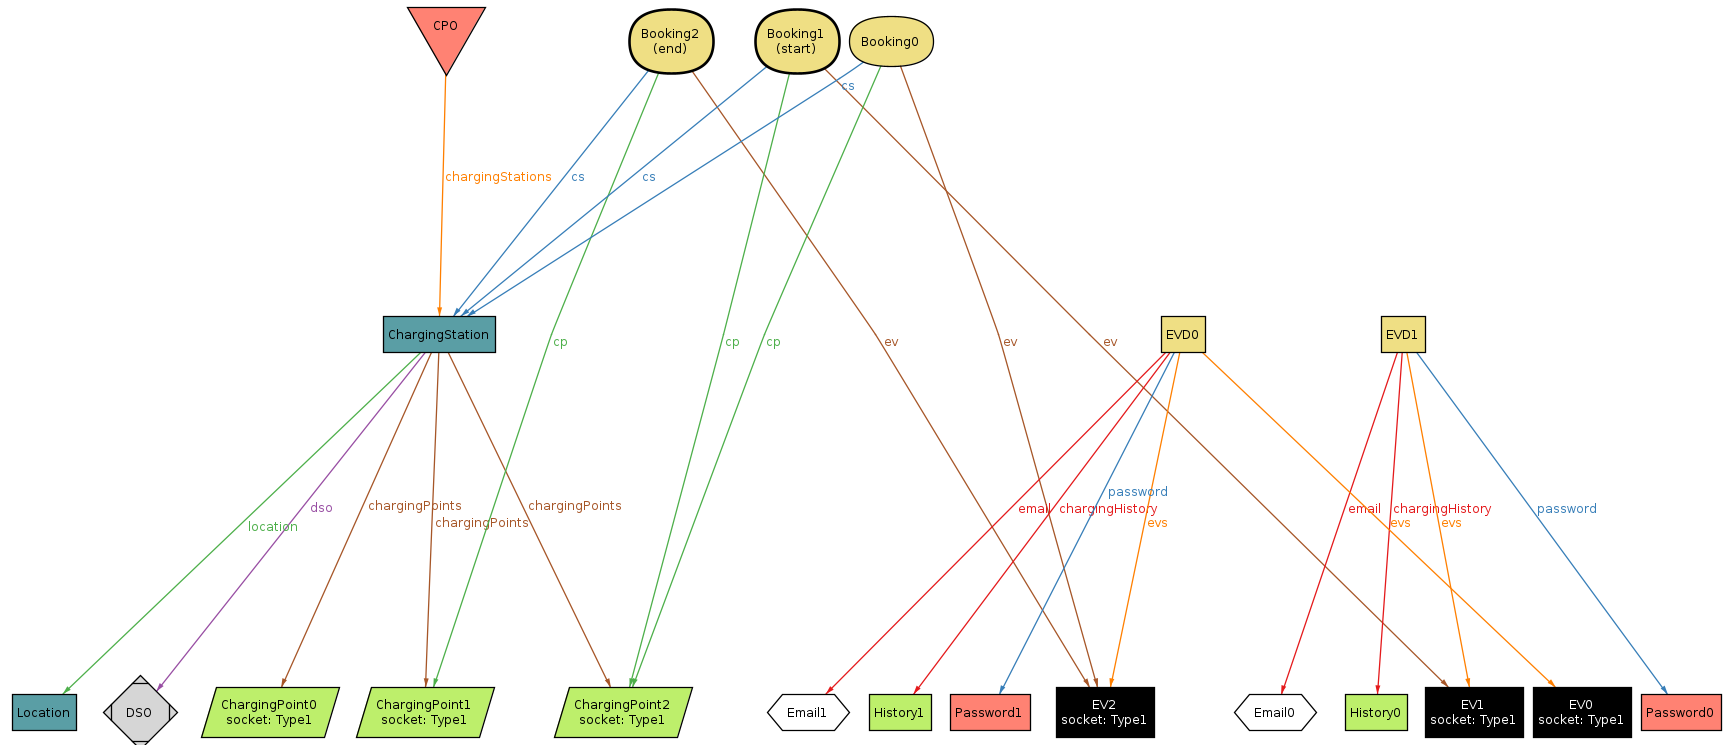
\includegraphics[width=1\textwidth]{Images/cp4/EVDWorldBooking.png}
    \caption{A first representation of the world from the EVD point of view}
\end{figure}

%TODO: in the Alloy add a time in using the charging point in the charge now case (free/occupied and in maintance CP?)
\begin{figure}[H]
    \centering
    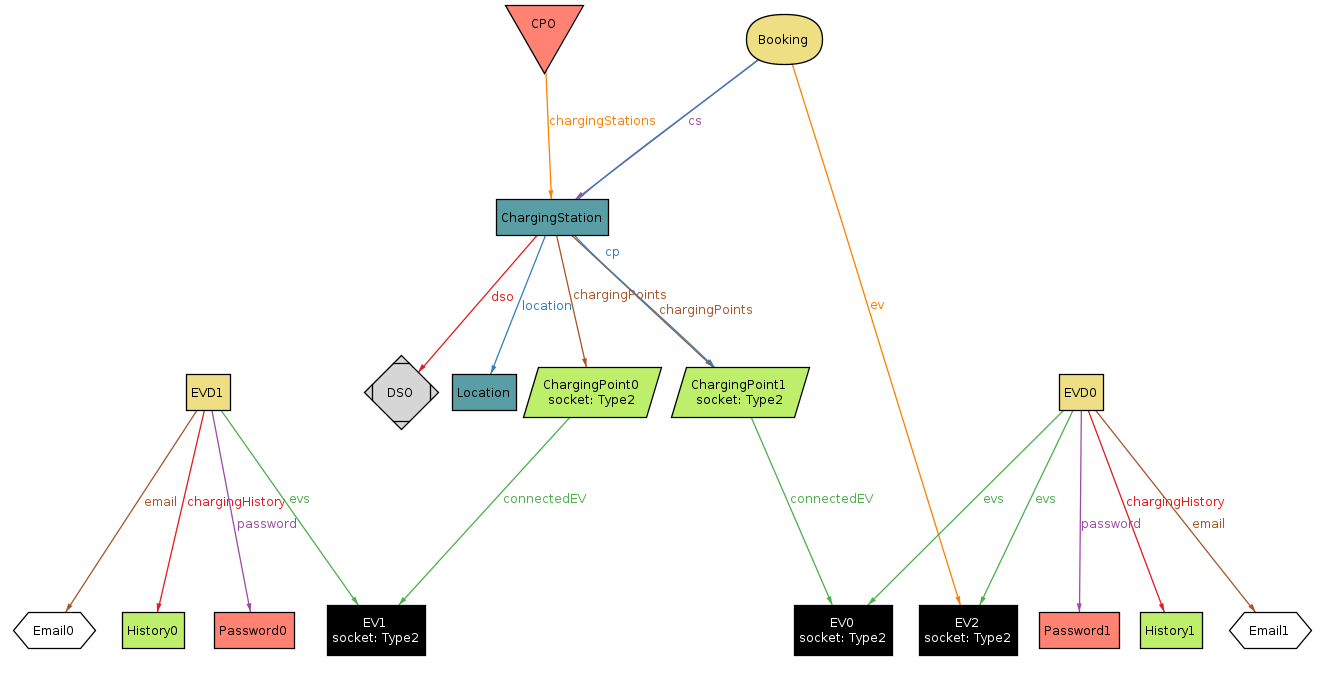
\includegraphics[width=1\textwidth]{Images/cp4/EVDWorldWithBookingAndChargeNow.png}
    \caption{A second representation of the world from the EVD point of view}
\end{figure}

Finally, we chose to show a dynamic model regarding the world that involves mainly the CPO. Running the predicate showAddCPToCS, explained in the Alloy code, we can see that a charging point is correctly added to the charging station related to the CPO that manages it.
\begin{figure}[H]
    \centering
    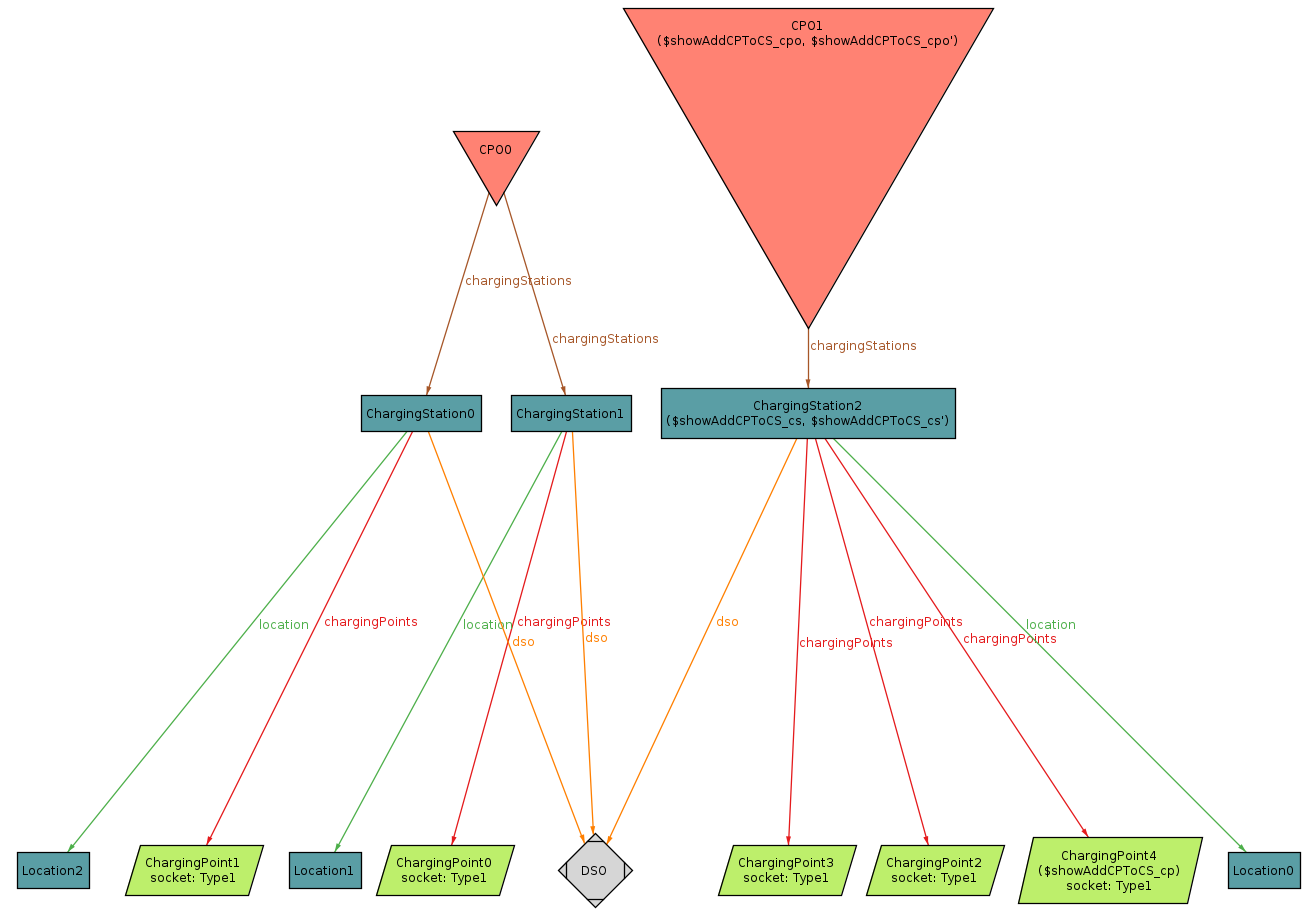
\includegraphics[width=1\textwidth]{Images/cp4/DynamicWorldAddCPToCS.png}
    \caption{A dynamic representation, considering the task of the CPO that ads a new charging point to a charging station}
\end{figure}